While the Texter processes the text information attached to the knowledge graph's entities, the Ruler exploits patterns in the graph structure to predict missing facts. Given an entity $x$ with a set of known facts $K$ containing facts of the form $(x, rel_k, tail_k)$ with $1 <= k <= |K|$ and $rel_k \in R$ and $tail_k \in E$ being any relation or entity, respectively, the Ruler leverages entity-related rules of the form $(x, rel_m, tail_m) <= (x, rel_k, tail_k)$ with $1 <= m <= |M|$ to predict a set of missing facts $M$. Therefore, the rules required for the inference process have to be mined from the knowledge graph, beforehand. That rule mining process can be viewed as the equivalent to the Texter's training process and some paragraphs in this thesis will refer to combined rule mining and creation of a Ruler as "training" a Ruler. Compatibel to the Texter, the Ruler is limited to the prediction of facts $(x, rel, tail)$ that contain the query entity as their head, as well. However, when the Ruler is applied to all entities $e \in E$, all facts of the form $(e, rel, x)$ are predicted at some point as far as the mined rules support it.

For rule mining, AnyBURL, the bottom-up rule mining algorithm, by Christian Meilicke et al.~\cite{Meilicke2019AnytimeBR} is used. It is an anytime algorithm, meaning that it can be interrupted anytime and still yield valid results. Bottom-up rule mining refers to the fact that the algorithm starts with concrete paths in the graph and tries to generalize those paths to rules instead of coming up with rules initially and searching for evidence later, which would be a top-down approach. Out of all possible Horn rules that might describe patterns in the graph, AnyBURL is restricted to rules that can be generalized from so-called \emph{ground path rules}. A ground path rule does not contain variables, but only constants, and must not contain any cycles in its body. Equation~\ref{eq:4_approach/2_ruler/ground_path_rule} describes the general form of a ground path rule of length $n$, meaning that it consists out of the head fact and $n$ body facts.

\begin{align}
(c_0, h, c_1)
    \Leftarrow (c_1, b_1, c_2), \dots, (c_n, b_n, c_{n+1}) &&
    c_k \neq c_l \forall k, l \in \{1, \dots, n+1\}, k \ne l
    \label{eq:4_approach/2_ruler/ground_path_rule}
\end{align}

Notably, despite the rule body being free of cycles, the ground path rule as a whole can still be cyclic if $c_0 = c_{n+1}$. Ground path rules are derived directly from randomly sampled paths in the graph and are subsequently generalized to rules that replace some of the constants with variables. If further supporting paths can be found for a general rule, it is kept. In their paper on AnyBURL, Meilicke et al. show that any rule that can be generalized from a ground path rules can be generalized to one of the three rule types formulated in Equations~\ref{eq:4_approach/2_ruler/c}~--~\ref{eq:4_approach/2_ruler/ac2}. Thereby, $C$-type rules can only be generalized from cyclic ground path rules, $AC2$ rules can only be generalized from acyclic ground path rules and $AC1$ can be generalized from both, cyclic and acyclic ground path rules. The following paragraphs outline the core algorihm used to mine such rules and derive some example rules from the small graph introduced in Chapter~\ref{ch:1_introduction}. Figure~\ref{fig:4_approach/2_ruler/rule_graph} shows an annotated subset of the graph that illustrates the rules. "Amsterdam" and "Netherlands" have been abbreviated to "AMS" and "NL" to keep the examples short.

\begin{align}
    C   && (Y, h, X)   &\Leftarrow (X, b_1, A_2), \dots, (A_n, b_n, Y)
    \label{eq:4_approach/2_ruler/c} \\
    AC1 && (c_0, h, X) &\Leftarrow (X, b_1, A_2), \dots, (A_n, b_n, c_{n+1})
    \label{eq:4_approach/2_ruler/ac1} \\
    AC2 && (c_0, h, X) &\Leftarrow (X, b_1, A_2), \dots, (A_n, b_n, A_{n+1})
    \label{eq:4_approach/2_ruler/ac2}
\end{align}

\begin{figure}[t]
    \centering
    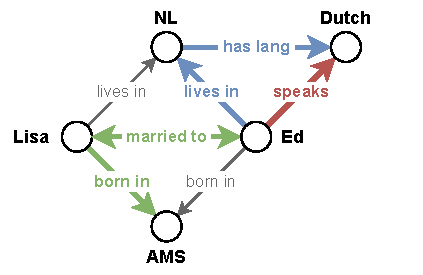
\includegraphics{4_approach/2_ruler/rule_graph}
    \caption{Subset of the previously introduced example graph with highlighted facts that form an acyclic (red + green) and a cyclic (red + blue) path}
    \label{fig:4_approach/2_ruler/rule_graph}
\end{figure}

Essentially, AnyBURL repeatedly samples random paths from the graphs, generalizes them to all possible rule types, looks for further paths that match the gained rules, and keeps those rules it finds further evidence for. For example, in search of rules of length 2, i.e. rules that have a body consisting of 2 facts, AnyBURL might randomly sample the two paths in~\ref{eq:4_approach/2_ruler/path_1} and~\ref{eq:4_approach/2_ruler/path_2} from the graph. Note, that parentheses denote entities, brackets denote relations and that the path does not need to follow directed edges in the graph. Furthermore, a close look at the paths reveals that the second path is cyclic as it starts and ends at the entity "Dutch".

\begin{align}
(Dutch)
    \leftarrow [speaks] - (Ed) - [married~to] \rightarrow (Lisa) - [born~in] \rightarrow (AMS)
    \label{eq:4_approach/2_ruler/path_1} \\
    (Dutch) \leftarrow [speaks] - (Ed) - [lives~in] \rightarrow (NL) - [has~lang] \rightarrow (Dutch)
    \label{eq:4_approach/2_ruler/path_2}
\end{align}

From those paths, AnyBURL would then derive the constant-only
ground path rules~\ref{eq:4_approach/2_ruler/acyclic_ground_path} and~\ref{eq:4_approach/2_ruler/cyclic_ground_path} by taking the path's first part as the rule's head and the remaining parts to form the rule's body.

\begin{align}
(Ed, speaks, Dutch)
    &\Leftarrow (Ed, married~to, Lisa), (Lisa, born~in, AMS)
    \label{eq:4_approach/2_ruler/acyclic_ground_path} \\
    (Ed, speaks, Dutch) &\Leftarrow (Ed, lives~in, NL), (NL, has~lang, Dutch)
    \label{eq:4_approach/2_ruler/cyclic_ground_path}
\end{align}

The acyclic ground path rule in~\ref{eq:4_approach/2_ruler/acyclic_ground_path} can be generalized to the $AC1$ rule~\ref{eq:4_approach/2_ruler/acyclic_ac1} and the $AC2$ rule~\ref{eq:4_approach/2_ruler/acyclic_ac2} while the cyclic ground path rule~\ref{eq:4_approach/2_ruler/cyclic_ground_path} can be generalized to the $C$ rule~\ref{eq:4_approach/2_ruler/cyclic_c} and the $AC1$ rule~\ref{eq:4_approach/2_ruler/cyclic_ac1}.

\begin{align}
    AC1 && (X, speaks, Dutch) &\Leftarrow (X, married~to, A_2), (A_2, born~in, AMS)
    \label{eq:4_approach/2_ruler/acyclic_ac1} \\
    AC2 && (X, speaks, Dutch) &\Leftarrow (X, married~to, A_2), (A_2, born~in, A_3)
    \label{eq:4_approach/2_ruler/acyclic_ac2} \\
        C   && (X, speaks, Y) &\Leftarrow (X, lives~in, A_2), (A_2, has~lang, Y)
    \label{eq:4_approach/2_ruler/cyclic_c} \\
    AC1 && (X, speaks, Dutch) &\Leftarrow (X, lives~in, A_2), (A_2, has~lang, Dutch)
    \label{eq:4_approach/2_ruler/cyclic_ac1}
\end{align}

Next, every rule candidate is scored by looking for further paths that match the rule's body and checking whether the graph also contains the fact predicted by the rule, i.e. whether the rule is correct in that case. Thereby, the number of paths that match the rule body is called the rule's \emph{support} while the ratio of times the rule is correct over its total support is called \emph{confidence}. Taking the cyclic rule~\ref{eq:4_approach/2_ruler/cyclic_c} as an example, AnyBURL would search for further evidence and find the path $(Lisa) - [lives~in] -> (NL) - [has~lang] -> (Dutch)$ that matches the rule body, increasing the rule's support to two, so far. However, the example graph does not contain the rule's predicted fact $(Lisa, speaks, Dutch)$, so the rule's support drops from 1 to $\frac{1}{2}$. Since rules that only apply to a single case or only once in every thousands case are not very useful, AnyBURL drops rules with a support of 1 or confidence below 0.0001 by default~\cite{AnyBURL}. It is noteworthy that, although some rules are more general than others, such as~\ref{eq:4_approach/2_ruler/acyclic_ac2} compared to~\ref{eq:4_approach/2_ruler/acyclic_ac1}, the more specific ones are still kept as they might end up with higher confidence for their special case during the ongoing mining process.

The process described by the above example is repeated until only few new rules of the same length $n$ can be found. AnyBURL then continues its search for rules of length $n + 1$ until it terminates after a fixed number of time steps. Listing~\ref{code:anyburl} shows the slightly adjusted pseudocode from the AnyBURL paper. The sampling and scoring process discussed above is implemented as the body of the inner while loop. The outer for loop implements the repeated check for the saturation of rules of the current length and the eventual proceeding to rules of increased length.

% TODO param s

\begin{listing}[t]
    \begin{lstlisting}
        AnyBURL(G, sat, Q, i, ts):
            n = 2
            R = $\emptyset$
            for i times:
                $R_s = \emptyset$
                start = current_time()
                while current_time() < start + ts:
                    p = sample_path(G, n)
                    $R_p$ = generate_rules(p)
                    for $r$ in $R_p$:
                        score($r$)
                        if $Q$($r)$:
                            $R_s$ = $R_s \cup {r}$

                $R_s^{'}$ = $R_s \cap R$
                if $|R_s^{'}| / |R_s| > sat$:
                    n = n + 1
                $R$ = $R \cup R_s$

            return $R$
    \end{lstlisting}
    \caption{The AnyBURL Rule Mining Algorithm taking a graph $G$ a saturation level $sat$, a quality criterion $Q$, and a number of iterations $i$, each of a timespan $ts$, as input and producing the ruleset $R$}
    \label{code:anyburl}
\end{listing}

A walk through the pseudocode reads as follows: Given the Graph $G$, the saturation threshold $s$, the quality criterion $Q$, a number of iterations $i$ and the timespan $ts$ each iteration endures, AnyBURL starts with an empty ruleset $R$, that will be extended after each iteration and returned in the end. The initial length of the randomly sampled paths is $n=2$, allowing to find the shortest possible rules of length 1. During the first iteration of duration $ts$, AnyBURL fills the rule set $R_s$, that keeps the rules found in the current iteration, by repeatedly sampling paths, generating rules from the paths, scoring the resulting rules, and keeping those with sufficient support and confidence. At the end of the iteration, when the timespan $ts$ has passed, $R_s^{'}$ is calculated as the set of rules mined during the iteration that were already known. If the share of already known rules mined during the current iteration exceeds the saturation threshold, the algorithm starts searching for rules of increased length. Otherwise, it continues with the current length. In both cases, the iteration's rules are added to the overall ruleset $R$. If the specified number of total iterations is reached, AnyBURL terminates and returns the mined rules $R$. In practice, AnyBURL saves the mined rules in a text file at the end and at configurable points during mining.

With the stored rules from AnyBURL in place, the Ruler is prepared for inference. Conceptually, given an entity and its known facts, the Ruler loads the rules, filters out further rules that do not meet the Ruler's quality demands and applies the remaining, useful rules to all known facts. All rules that can be applied successfully are kept together with their confidence. From all the facts predicted by the applied rules, already known facts from the existing graph are filtered out. The remaining facts are sorted by confidence and returned to the user - together with the rules that predicted them as an explanation for the user. If multiple rules predict the same fact, the fact is assigned the highest confidence of those rules and is returned together with all of them. The Ruler's extra quality criterion mentioned above further restricts the considered rules to those with confidence greater 50\%, because AnyBURL's minimum confidence threshold of 0.01\% allows many rules that predict false positives. For open-world entities, this algorithm implies an empty result set as no rule can cover an entity that is not connected to any other entity and all the facts predicted for the train entities will be filtered out. In those cases, the Power model has to rely solely on the Texter.
